\documentclass[a4paper]{article}

\usepackage{acronym}
\usepackage[intoc]{nomencl}
\usepackage{todonotes}
\usepackage{listings}
\usepackage{color}
\usepackage{amsmath}
\usepackage{amsfonts}
\usepackage{acronym}
\usepackage{bytefield}
\usepackage{marvosym}
\usepackage[pdftex,
		pdfauthor={Roel Baardman},
		pdftitle={Transponder check}]{hyperref}
		


\definecolor{dkgreen}{rgb}{0,0.6,0}
\definecolor{gray}{rgb}{0.5,0.5,0.5}
\definecolor{mauve}{rgb}{0.58,0,0.82}

\lstset{	keywordstyle=\color{blue},
		commentstyle=\color{dkgreen},
		stringstyle=\color{mauve},
		numbers=left,
		numberstyle=\tiny\color{gray},
		stepnumber=2,
		numbersep=5pt,
		breaklines=true,
		breakatwhitespace=false,
		title=\lstname
}


\graphicspath{{img/}}

\begin{document}
The maintainance manual of PH-1516\cite{AMP_PH1516} references MD NL-2011-002 R1, due to the existance of a transponder installation.

The Dutch government writes in MD NL-2011-002 R1\cite{NL_2011_002_R1}, Appendix A, Table 1, Footnote 3: \emph{``Refer to EC Regulation 1207/2011 article 7(2) for mandatory periodic testing of Mode S Transponder systems.''}

EC Regulation 1207/2011\cite{EC_1207_2011} article 7(2) states: \emph{``Operators shall ensure that a check is performed at least every two years, and, whenever an anomaly is detected on a specific aircraft, so that the data items set out in point 3 of Part A of Annex II, in point 3 of Part B of Annex II and in point 2 of Part C of Annex II, if applicable, are correctly provided at the output of secondary surveillance radar transponders installed on board their aircraft. If any of the data items are not correctly provided then the operator shall investigate the matter before the next flight is initiated and any rectification necessary shall be introduced in line with normal maintenance and corrective procedures for the aircraft and its avionics.''}

EASA SIB 2011-15R2, Appendix 1 states:
\begin{itemize}
\item[a.]{When not required, ensure all transponders are selected to ‘OFF’ or ‘Standby’.}
\item[b.]{Before starting any test, contact the local Air Traffic Control Unit and advise them of your intention to conduct transponder testing. Advise the Air Traffic Unit of your start time and test duration. Also inform them of the altitude(s) at which you will be testing, your intended Aircraft Identification (Flight Id) and your intended Mode A code. See para c and d. Note: Certain altitudes may not be possible due to over flying aircraft.}
\item[c.]{Set the Mode A code to 7776 (or other Mode A code agreed with Air Traffic Control Unit). Note: The Mode A code 7776 is assigned as a test code by the ORCAM Users Group, specifically for the testing of transponders.}
\item[d.]{For Mode S equipped aircraft, set the Aircraft Identification (Flight Id) with the first 8 characters of the company name. This is the name of the company conducting the tests.}
\item[e.]{For Mode S equipped aircraft, set the on-the-ground status for all Mode S replies, except when an airborne reply is required (e.g. for altitude testing).}
\item[f.]{Where possible, perform the testing inside a hanger to take advantage of any shielding properties it may provide.}
\item[g.]{As a precaution, use antenna transmission covers whether or not testing is performed inside or outside.}
\item[h.]{When testing the altitude (Mode C or S) parameter, radiate directly into the ramp test set via the prescribed attenuator.}
\item[i.]{In between testing, i.e. to transition from one altitude to another, select the transponder to ‘standby’ mode.}
\item[j.]{If testing transponder parameters other than ‘altitude’, set altitude to -1000 feet (minus 1000 feet), or over 60000 feet. This will minimise the possibility of ACAS warning to airfield and overflying aircraft.}
\item[k.]{When testing is complete select the transponder(s) to ‘OFF’ or ‘Standby’.}
\end{itemize}


\section{Test setup}
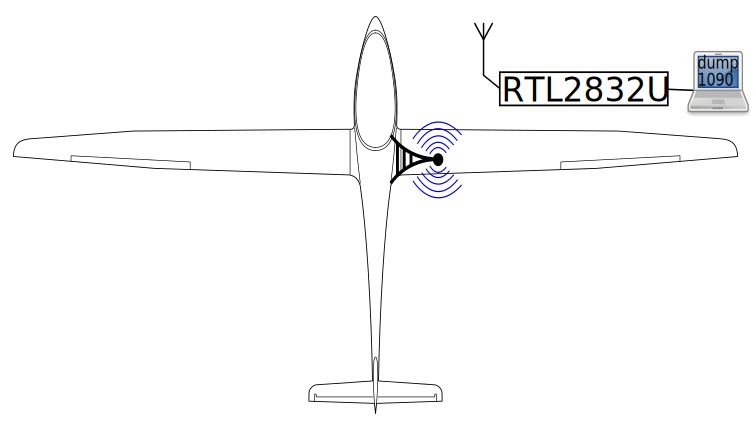
\includegraphics[width=\textwidth]{setup}

\bibliographystyle{ieeetr}
\bibliography{references}


\end{document}
